% Chapter 2
\makeatletter
\def\input@path{{../}}
\makeatother
\documentclass[../main.tex]{subfiles}
\begin{document}
\chapter{Methods} % Chapter title

\label{ch:methods} % For referencing the chapter elsewhere, use \autoref{ch:examples} 

%----------------------------------------------------------------------------------------

This Chapter establishes research methods applied in the thesis. Section \ref{ch2s1} introduces Burgers vortex analytical model and provides literature review for adjusting model parameters. Section \ref{ch2s2} presents the basics of dynamical systems formalism and  brings concepts used for describing the single particle motion in a model of a vortex.  Section \ref{ch2s3} makes a preliminary analysis of the particle equation of motion, tracks the steps to its numerical solution and sets the assumptions for the proper, multiple particle model specific for this thesis. Section \ref{ch2s4} is devoted to experimental techniques and observation details. Last, but not least, Section \ref{ch2s5} collects the data on the properties of cloud droplets and cloud turbulence, to establish "cloud-like" conditions that are applied in numerical simulations.

\section{Vortex model}
\label{ch2s1}
A model of intense vortex structure chosen for the analysis is Burgers vortex with stretching \citep{Burgers1948}. It is exact, axisymmetric, steady solution to NSE and a product of balance between stretching effect and viscous diffusion \citep{Perry1987}. It is commonly used as an approximation of a vortex tube in DNS and laboratory experiments \citep{Neu1984, Jimenez1998, Bellin1999}. Despite its simplicity and limited connection to 3D turbulence, Burgers vortex serves as a testing ground for many physical and mathematical ideas.\\
Burgers vortex is a 3D steady velocity field $\vec{u}$ determined by two parameters: \emph{circulation} $\Gamma$ and \emph{stretching strength} $\gamma$. The irrotational motion sweeps vorticity radially inward while simultaneously straining the vortex tube in the axial direction, as presented schematically in Fig. \ref{fig:ch2_01a}. These processes exactly counterbalance the tendency for vorticity to diffuse radially outward and as a result it is constant in time.
\begin{figure*}
\centering
\noindent 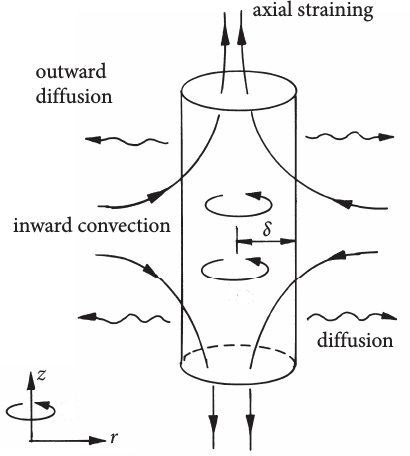
\includegraphics[width=20pc]{gfx/Burg_vortex_scheme.png}
\caption{Straining of vorticity in Burgers vortex. $\delta$ is vortex core size  (from \citet{Davidson2004}).}
\label{fig:ch2_01a}
\end{figure*}
If vortex axis is aligned with $z$-axis in the cylindrical coordinate system $(r, \varphi, z)$, then its vorticity:
\begin{equation}
\vec{\omega}=\frac{\Gamma}{2 \pi \delta^2} e^{-\frac{r^2}{2 \delta^2}} \hat{e}_z
\label{def:omega_Bur}
\end{equation}
and velocity field:
\begin{equation}
\vec{u}=-\frac{\gamma}{2} r \hat{e}_r+\frac{\Gamma}{2 \pi r} \left(1-e^{-\frac{r^2}{2\delta^2}}\right)\hat{e}_{\varphi}+\gamma z \hat{e}_z,
\label{def_Bur}
\end{equation}
where $\delta=\sqrt{2 \nu / \gamma}$ is the \emph{vortex core size}.\marginpar{vortex core size} The characteristic timescale of the Burgers vortex flow, vortex core \emph{turnover time}, is:\marginpar{vortex turnover time}
\begin{equation}
\tau_f=\delta^2 \Gamma^{-1}
\label{def:tau_f}
\end{equation}

By the definition, azimuthal velocity reaches its maximum at $r=r_s \delta$, where $r_s=const$, so the definition introduces a spatial scale $r_s$ into the system. Precise analytical formulation is such, that $r_s=\sqrt{-2 W(1,-exp(-1/2)/2)-1}$, where $W(k,x)$ denotes Lambert W functions' $k$-th branch of $x$. For the purposes of this thesis, only the numerical estimation is used: $r_s \approx 1.5852011$. Burgers vortex velocity components scaled with vortex spatial and time scales, $\delta$ and $\tau_f$, are:
\begin{equation}
\vec{u^+}=- A r^+ \hat{e}_r+\frac{1}{2 \pi r^+} \left(1-e^{-\frac{r^{+ 2}}{2}}\right)\hat{e}_{\varphi}+ 2 A z^+ \hat{e}_z
\label{def:Bur_nodim}
\end{equation}
where $A=Re_{\nu}^{-1}$ is vortex strain parameter, defined later in the text, and $^+$ denotes dimensionless variables. Three dimensionless velocity components are plotted in Fig.\ref{fig:ch2_01b} for $A=0.001$.
\begin{figure*}
\centering
\noindent 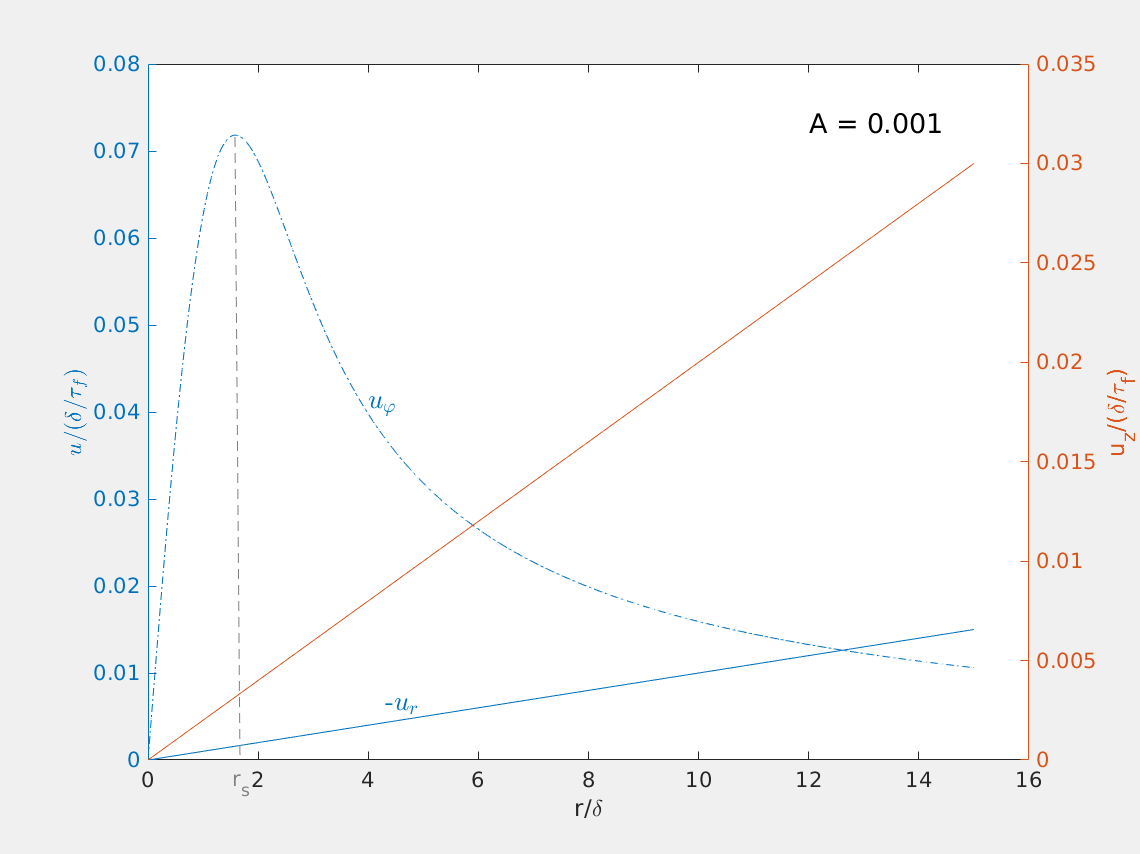
\includegraphics[width=30pc]{gfx/Burg_vor_vel_comp.png}
\caption{Burgers vortex dimensionless velocity components in cylindrical coordinates for arbitrary strain parameter $A=0.001$. $r_s$ is defined in the text.}
\label{fig:ch2_01b}
\end{figure*}

In order to adjust the model to atmospheric turbulence application, one needs to calibrate model parameters. Past theoretical and experimental studies lack general conclusions about vortex characteristic time and length scales, intensity and appearance in turbulence. Most of this inconclusive information that is availabe is summarised here. Statistical analysis of DNS data \citep{Jimenez1998, Bellin1999, Moisy2004, Pirozzoli2012}) and of experimental data \citep{Mouri2003} indicate that Burgers vortex core size $\delta$ has a log-normal probability distribution. It scales roughly with the Kolmogorov length scale: $\delta= m\eta$ and $m$ range varies in different papers. Generally its minimum reaches 1 and maximum around 12-22. The mean values fall into the range $\langle m \rangle = 3-7$. \citet{Jimenez1998} estimates the length of a tube and claim that it scales as $\simeq Re_{\lambda}^{1/2}$. All these studies had relatively low Reynolds number: $Re_{\lambda} \simeq 100-1000$. \citet{Bellin1999} reports that the vortex Reynolds number is $Re_v=\Gamma/\nu \approx 200-400$ . This reaserch, among other papers, shows that azimuthal velocity decreases much faster far from the axis then in Burgers vortex model. \citet{Pirozzoli2012} investigated this issue as well, but in more detail. \citet{Moisy2004} analyzing DNS instant velocity fields propose that vorticity structures’ geometrical aspect ratios evolve towards long tubes (1 : 1 : 10), while increasing vorticity threshold. In the study by \citet{Biferale2010}, statistics of vortex filament lifetime for a low Taylor microscale Reynolds number $Re_{\lambda}$ indicate that the maximum lifetime is on the order of the integral timescale, whereas its mean lifetime scales with the Kolmogorov timescale. Many of the works cited here suggest that there is a relation between root mean square velocity fluctuations $\bar{u'}$ and the circulation parameter $\Gamma$.

Tu dodac jeszcze jedna informacje o skalowaniu.

\section{Dynamical systems formalism}
\label{ch2s2}
Dynamical systems theory includes an extensive body of
knowledge about qualitative properties of generic smooth
families of vector fields and discrete maps. The theory abandons the goal of describing the qualitative dynamics of all systems as hopeless and instead restricts its attention to phenomena that are found in selected systems. Here are presented the dynamical phenomena that are relevant to deterministic system of a single particle moving in Burgers vortex as determined by Eq.\ref{ch1:eq04}.\\
Topological features of a dynamical system - singularities, periodic orbits, and the ways in which the orbits intertwine - are invariant under a general continuous change of coordinates. Equilibria and periodic orbits are flow invariant sets. Local quantities such as the eigenvalues of equilibria and periodic orbits, and global quantities such as Lyapunov exponents, metric entropy, and fractal dimensions are examples of properties of dynamical systems independent of coordinate choice. That is why these quantities are good descriptors of flow structure. The definitions of several of the above are given below.\\
\marginpar{dynamical system}
A \emph{dynamical system} is a triple $\{M,f,T\}$ consisting of manifold $M$ called the phase (or state) space endowed with a family of smooth evolution functions $f^t$ that for any time $t \in T$ map the manifold into itself: $f^t : M \mapsto M$. In the case of continous-time dynamical system and real time $t \in \Re$, the family $\{f^t\}_{t\in T}$ of evolution operators is called a \emph{flow} (under additional conditions). A \emph{flow map} for a given $t$ transforms a state vector $\mathbf{x_0} \in M$ into another state vector $\mathbf{x} \in M$:
\begin{equation}
f^t : \mathbf{x_0} \mapsto \mathbf{x}(\mathbf{x_0},t)
\label{def:flowmap}
\end{equation}
\marginpar{trajectory and orbit}A sequence of points $\mathbf{x}(t) = f^t(\mathbf{x_0})$ for $t$ in finite range is called the \emph{trajectory} through the point $\mathbf{x_0}$. A trajectory can be stationary, periodic or aperiodic. An \emph{orbit} refers to totality of states that can be reached from the point $\mathbf{x_0}$.\\
Continuous dynamical system can be written as system of coupled ordinary differential equations. When a dynamial system is represented by a set of equations $\dot{\mathbf{x}}(t)=\mathbf{v}(\mathbf{x},t)$, then $\mathbf{v}(\mathbf{x},t)$ is called a \emph{generalized velocity field}.\\
\marginpar{equillibrium point}\emph{Equillibrium point} $\mathbf{x_k}$ (also referred to as a stationary, fixed, critical, invariant, rest, stagnation)  is a state vector for which $\vee t \ v(\mathbf{x_k},t)=0$ (equivalently $\vee t \ f^t : \mathbf{x_k} \mapsto \mathbf{x_k}$).\marginpar{periodic orbit} A \emph{periodic orbit/cycle} $p$ is the set of points $M_p \subset M$ swept out by a trajectory that returns to the initial point in a finite time.\\
\marginpar{attractor} An \emph{attractor} $\Omega$ is a subset of $M$ onto which a flow is contracting i.e. there exists a connected state space volume that maps into itself under forward evolution. The attractor may be unique, or there can coexist any number of distinct attracting sets, each with its own \emph{basin of attraction} - the set of all points that fall into the attractor under
forward evolution. The attractor can be a fixed point (a sink), a periodic orbit (a limit cycle), aperiodic, or any combination of the above. Conversely, if we can enclose a set $\Omega$ by a connected state space volume $M_0 \subset M$ and then show that almost all points within $M_0$, but not in $\Omega$, eventually exit $M_0$, we refer to $\Omega$ as a \emph{repeller}.\marginpar{repeller}\\
The state space $M$ is stratified into a union of orbits. In order to understand the dynamics of the system it is enough to understand how $M$ is stratified and to grasp the nature of its orbits. The central term in this process is stability. Stability matrix is a basic tool characterizing the stability of an orbit:
\begin{equation}
A_{ij}(\mathbf{x})\equiv \frac{\partial}{\partial \mathbf{x_j}}(\mathbf{v_i}(\mathbf{x}))
\label{def:stab_mat}
\end{equation}
where $\mathbf{x}=\mathbf{x}(\mathbf{x_0},t)$ is a trajectory. It expresses the rate of the infinitesimal neighbourhood deformation along the trajectory. However to get to know finite time deformation needed for stability analysis, one needs to know the Jacobian matrix $J^t$. Its relations to stability matrix are provided here only for the cases of interest to this thesis: equillibrium points and periodic orbits.\\
For equillibrium point $\mathbf{x_k}$ the Jacobian matrix is:
\begin{equation}
J^t(\mathbf{x_k})=e^{A(\mathbf{x_k})t}
\label{def:Jacobian}
\end{equation}
hence the stability of equillibrium point $\mathbf{x_k}$ is determined by eigenvalues of stability matrix $\lambda^{(l)}_k=a^{(l)}_k+ib^{(l)}_k$. Assuming
that these eigenvalues are non-degenerate, $\lambda^{(l)} \neq \lambda^{(m)}$ for any pair of eigenvalues, the following claims are present.

\begin{itemize}
\item If all $a^{(l)} < 0$, then the equilibrium is stable - a \emph{sink}. For $b^{(l)} = 0$, it is an \emph{stable node}; for $b^{(l)} \neq 0$, it is an \emph{stable spiral/focus}.
\item If some $a^{(l)} < 0$, and other $a^{(l)} > 0$, the equilibrium is hyperbolic, or a \emph{saddle}.
\item If all $a^{(l)} > 0$, then the equilibrium is repelling, or a \emph{source}. For $b^{(l)} = 0$, it
is an \emph{unstable node}; for $b(j) \neq 0$, it is an \emph{unstable spiral/focus}.
\item If $\det A(x_k)=0$, $tr A(x_k) \neq 0$ it is neutral, a \emph{center} (elliptic).
\item If some $a^{(l)} = 0$ there is a symmetry or a bifurcation.
\end{itemize}
Figures \ref{fig:ch2_02} and \ref{fig:ch2_03} show diagrams of number of equillibrium point examples. It is important to realise that these examples are pictured in phase space, not in real space.
\begin{figure*}
\centering
\noindent 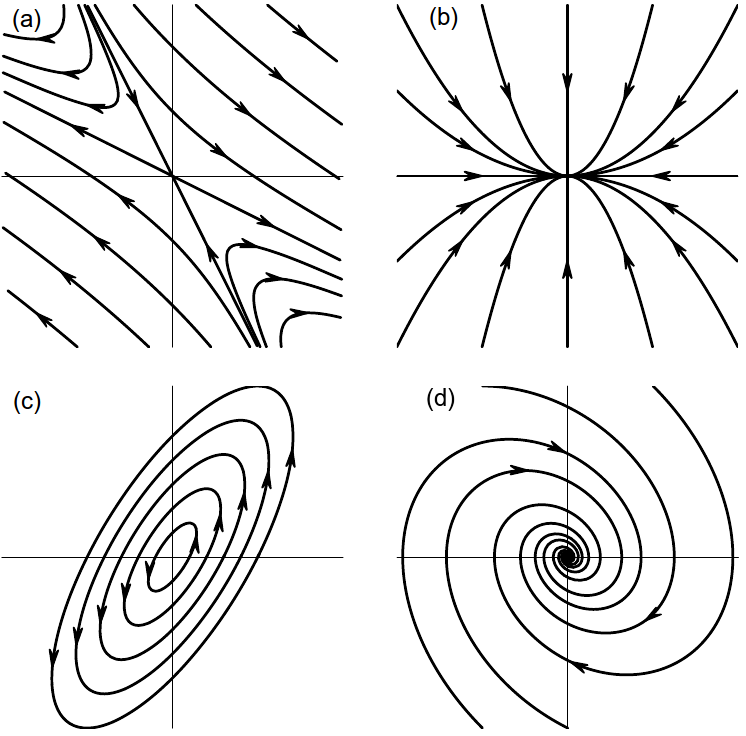
\includegraphics[width=20pc]{gfx/eq_stability_2D.png}
\caption{Trajectories in linearized neighborhoods
of several 2-dimensional equilibria: (a) saddle (hyperbolic), (b) stable node (attracting), (c) center (elliptic), (d) stable spiral (from \citet{ChaosBook}).}
\label{fig:ch2_02}
\end{figure*}

\begin{figure*}
\centering
\noindent 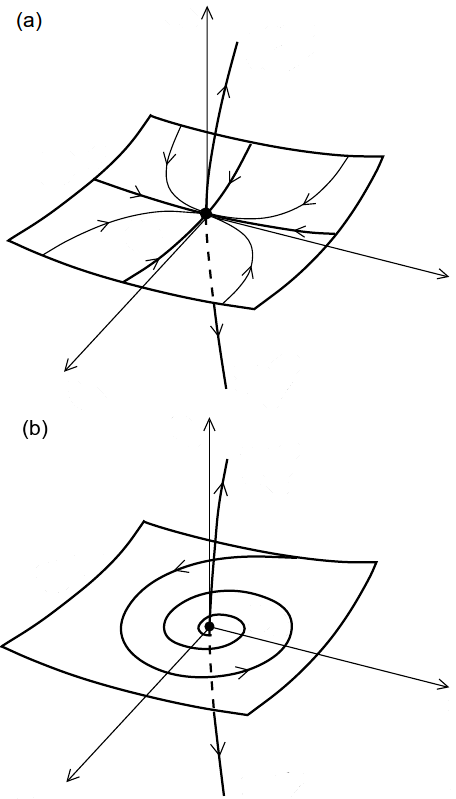
\includegraphics[width=20pc]{gfx/eq_stability_3D.png}
\caption{Trajectories in linearized neighborhoods
of 3-dimensional equilibria: (a) saddle, (b) saddle-focus.}
\label{fig:ch2_03}
\end{figure*}

A periodic orbit of a continuous-time flow can be:
\begin{itemize}
\item stable, a sink or a \emph{limit cycle},\marginpar{limit cycle} 
\item hyperbolic or a saddle, unstable to perturbations outside its stable manifold,
\item elliptic, neutral or marginal,
\item partially hyperbolic,
\item repelling, or a source, unstable to any perturbation
\end{itemize}
The range of system parameter values for which a periodic orbitis stable is called its \emph{the stability window}. The set of initial points that are asymptotically attracted to stable periodic orbit in infinity (for a fixed set of system parameter values) is called \emph{the basin of attraction} of the limit cycle. For the detailed analysis of periodic orbit stability conditions see \citep{ChaosBook}.\\
\emph{Bifurcation} is a change of the topological type of the system as its parameters pass through a \emph{bifurcation (critical) value}. One of the classes of bifurcations is so called \emph{Hopf bifurcation} \citep{Kuznetsov2004}. \marginpar{Hopf bifurcation}Suppose $\alpha$ is a bifurcation parameter and $\alpha_{cr}=0$ is the critical value. In Hopf bifurcation, for $\alpha \leq 0$ the equilibrium is a stable focus. If $\alpha > 0$ the equilibrium becomes an unstable focus and the system has a stable periodic orbit. This is presented schematically in Fig.\ref{fig:ch2_04}.

\begin{figure*}
\centering
\noindent 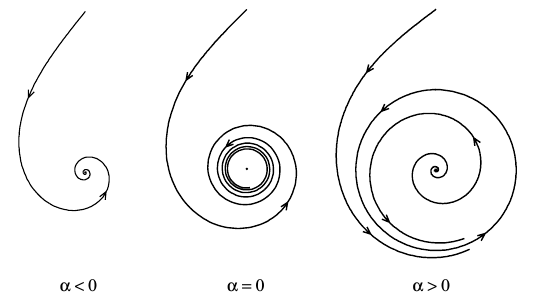
\includegraphics[width=20pc]{gfx/Hopf_bifur.png}
\caption{Hopf bifurcation depicted in a plane. $\alpha$ is bifurcation parameter, its critical value is $\alpha_{cr}=0$. The figure comes from \citep{Kuznetsov2004}.}
\label{fig:ch2_04}
\end{figure*}

In order to use the methodology described above to analyze the motion of a particle in a vortex of axial symmetry, it is necessary to first define the state space. When choosing a cylindrical coordinates in $\Re^3$ the position vector is $\vec{r}=\vec{r}(r,\varphi,z)$, the state vector is $\mathbf{x}=(r,\varphi,z,\dot{r},\dot{\varphi},\dot{z})$ and generalized velocity $\mathbf{v}=(\dot{r},\dot{\varphi},\dot{z},\ddot{r},\ddot{\varphi},\ddot{z})$.\\

\section{Numerical simulations}
\label{ch2s3}

 \subsection{Single particle trajectory}
Solving Eq.\ref{ch1:eq04}, the equation of particle motion, for arbitrary parameters and initial conditions, even in steady vortex flow as defined in \ref{def:Bur} requires numerical calculations. Below are described the consecutive steps needed to perform these calculations. First few steps of the procedure are also of use for analytical analysis.\\
In the rectangular coordinate system, in which $z$ axis is aligned with vortex axis, gravity force vector, without loss of generality, is defined to be inclined by the arbitrary angle $\theta \in (0, 90^o]$ to vortex axis:
\begin{equation}
\vec{g}=-g\left(\sin\theta \hat{e_y}+\cos\theta\hat{e_z}\right)
\end{equation}
where $g$ is gravitational constant. In cylindrical coordinates:
\begin{align}
\vec{g}/g=-\sin{\theta} \sin{\varphi} \hat{e_r}-\sin{\theta} \cos{\varphi}\hat{e_{\varphi}}-\cos{\theta} \hat{e_z},\\\ddot{\vec{r}}=(\ddot{r}-r \dot{\varphi}^2) \hat{e_r}+(2 \dot{r} \dot{\varphi} +r \ddot{\varphi})\hat{e_{\varphi}}+\ddot{z} \hat{e_z}.
\label{ch2:eq01}
\end{align}
Equation \ref{ch1:eq04} decomposed into components looks therefore as follows:
\begin{align}
\ddot{r}-r \dot{\varphi}^2=\tau_p^{-1}\left(-\gamma r/2-\dot{r} \right)-g \sin{\theta} \sin{\varphi}\\
2 \dot{r} \dot{\varphi} +r \ddot{\varphi} = \tau_p^{-1}\left( \frac{\Gamma}{2 \pi r} \left(1-\exp(-\gamma r^2/4\nu)\right)-r\dot{\varphi}\right) - g \sin{\theta} \cos{\varphi}\\
\ddot{z}=\tau_p^{-1}\left(\gamma z - \dot{z}\right) - g \cos{\theta}
\label{ch2:eq02}
\end{align}
The system is primarely dependent on a set of six dimensional parameters: $\{\Gamma, \gamma, \theta, \tau_p, g, \nu \}$. The non-dimensionalization however leads to Eq. \ref{ch3:eq03a}-\ref{ch3:eq03c} and gives a set of 4 dimensionless parameters $\{St, S_v, \theta, A \}$. to be defined below Dimensionless variables are denoted henceforth by $^{+}$.

\begin{align}
\ddot{r^+}-r^+\dot{\varphi^+}^2=-St^{-1}\left(A r^++\dot{r^+}+S_v \sin\varphi\right) \label{ch2:eq03a} \\
2\dot{r^+}\dot{\varphi^+}+r^+\ddot{\varphi^+}=St^{-1}\left(\frac{1}{2 \pi r^+}(1-e^{-\frac{r^{+ 2}}{2}})-r^+\dot{\varphi^+}-S_v\cos\varphi\right) \label{ch2:eq03b} \\
\ddot{z^+}=St^{-1}\left(A z - \dot{z^+} - S_v \cot\theta\right) \label{ch2:eq03c}
\end{align}

\noindent A quantity $A=\nu \Gamma^{-1}=Re_v^{-1}$ is the dimensionless strain parameter\marginpar{vortex strain parameter}, the inverse of vortex Reynolds number $Re_v$. Stokes number here is calculated with the use of vortex turnover time $\tau_f$ so $St=\nu \tau_p A^{-1} \delta^{-2}$. The sedimentation parameter is $S_v=\nu^{-1} g A \delta \tau_p \sin\theta $. It characterizes the motion in a plane perpendicular to the vortex axis ($r,\varphi$), that is called here \emph{2D space}. As one can see the equation describing particle motion along the vortex axis (Eq. \ref{ch3:eq03c}) are independent from the equations describing motion in 2D space (Eq.\ref{ch3:eq03a}, \ref{ch3:eq03b}), i.e.they depend on different variables. Thus they can be solved separately. The analysis of single droplet motion using similar formalism was conducted by \citet{Marcu1995}.\\
The set of equations \ref{ch2:eq03a}-\ref{ch2:eq03c} is used next to transcribe the state vector evolution:
\begin{gather}
\dot{\mathbf{x^+}}=\frac{d}{dt^+}
\begin{bmatrix} r^+\\ \varphi\\ z^+\\ \dot{r^+}\\ \dot{\varphi^+}\\ \dot{z^+}\\
\end{bmatrix}
=
\begin{bmatrix} \dot{r^+} \\\dot{\varphi^+}\\ \dot{z^+} \\ 
-M_1 r^+/2-M_2 \dot{r^+} -M_3 \sin{\varphi^+}+r\dot{\varphi^+}^2 \\
M_2\left( 1-\exp(-r^{+ 2}/2)-\right)/2 \pi r^{+ 2}-M_3 \cos{\varphi^+}/r^+ -2\dot{r^+}\dot{\varphi^+}/r^+-M_2\dot{\varphi^+}\\
M_1 z^+-M_2 \dot{z^+} - M_4
\end{bmatrix}
\label{ch02:eq04}
\end{gather}
while for convenience, new equation parameters are defined:
\begin{align}
M_1=\frac{2A}{St}=\frac{\tau_p}{\gamma^{-1}}St^{-2},\\ \nonumber
M_2=St^{-1},\\ 
M_3=Fr^{-2},\\ \nonumber
M_4=Fr^{-2} \cot{\theta}. \nonumber
\label{def:Mrs}
\end{align}
In such a form the set of dimensionless equations (Eq. \ref{ch02:eq04}) is solved numerically in Matlab environment by \emph{ode45} build in solver, which is based on an explicit Runge-Kutta (4,5) formula, the Dormand-Prince pair. It is a single-step solver and it uses adaptive time steps. Relative error tolerance assumed is $10^{-3}$, absolute error tolerance is $10^{-6}$.

\subsection{Multiple particles in vortex domain}
 
To imitate processes occurring in clouds and examine the effect exerted on a droplet field by the presence of a vortex, a 3D vortex model was designed. Its domain is cylindrical in shape, of radius $D$ and half-length $Z$ (see Fig. \ref{fig:ch2_05}). Initially the domain is filled uniformly with a given number concentration $n$ of particles. No interaction between droplets is imposed. During the course of simulation, particles leaving the simulation domain are removed.

\begin{figure*}
\centering
\noindent 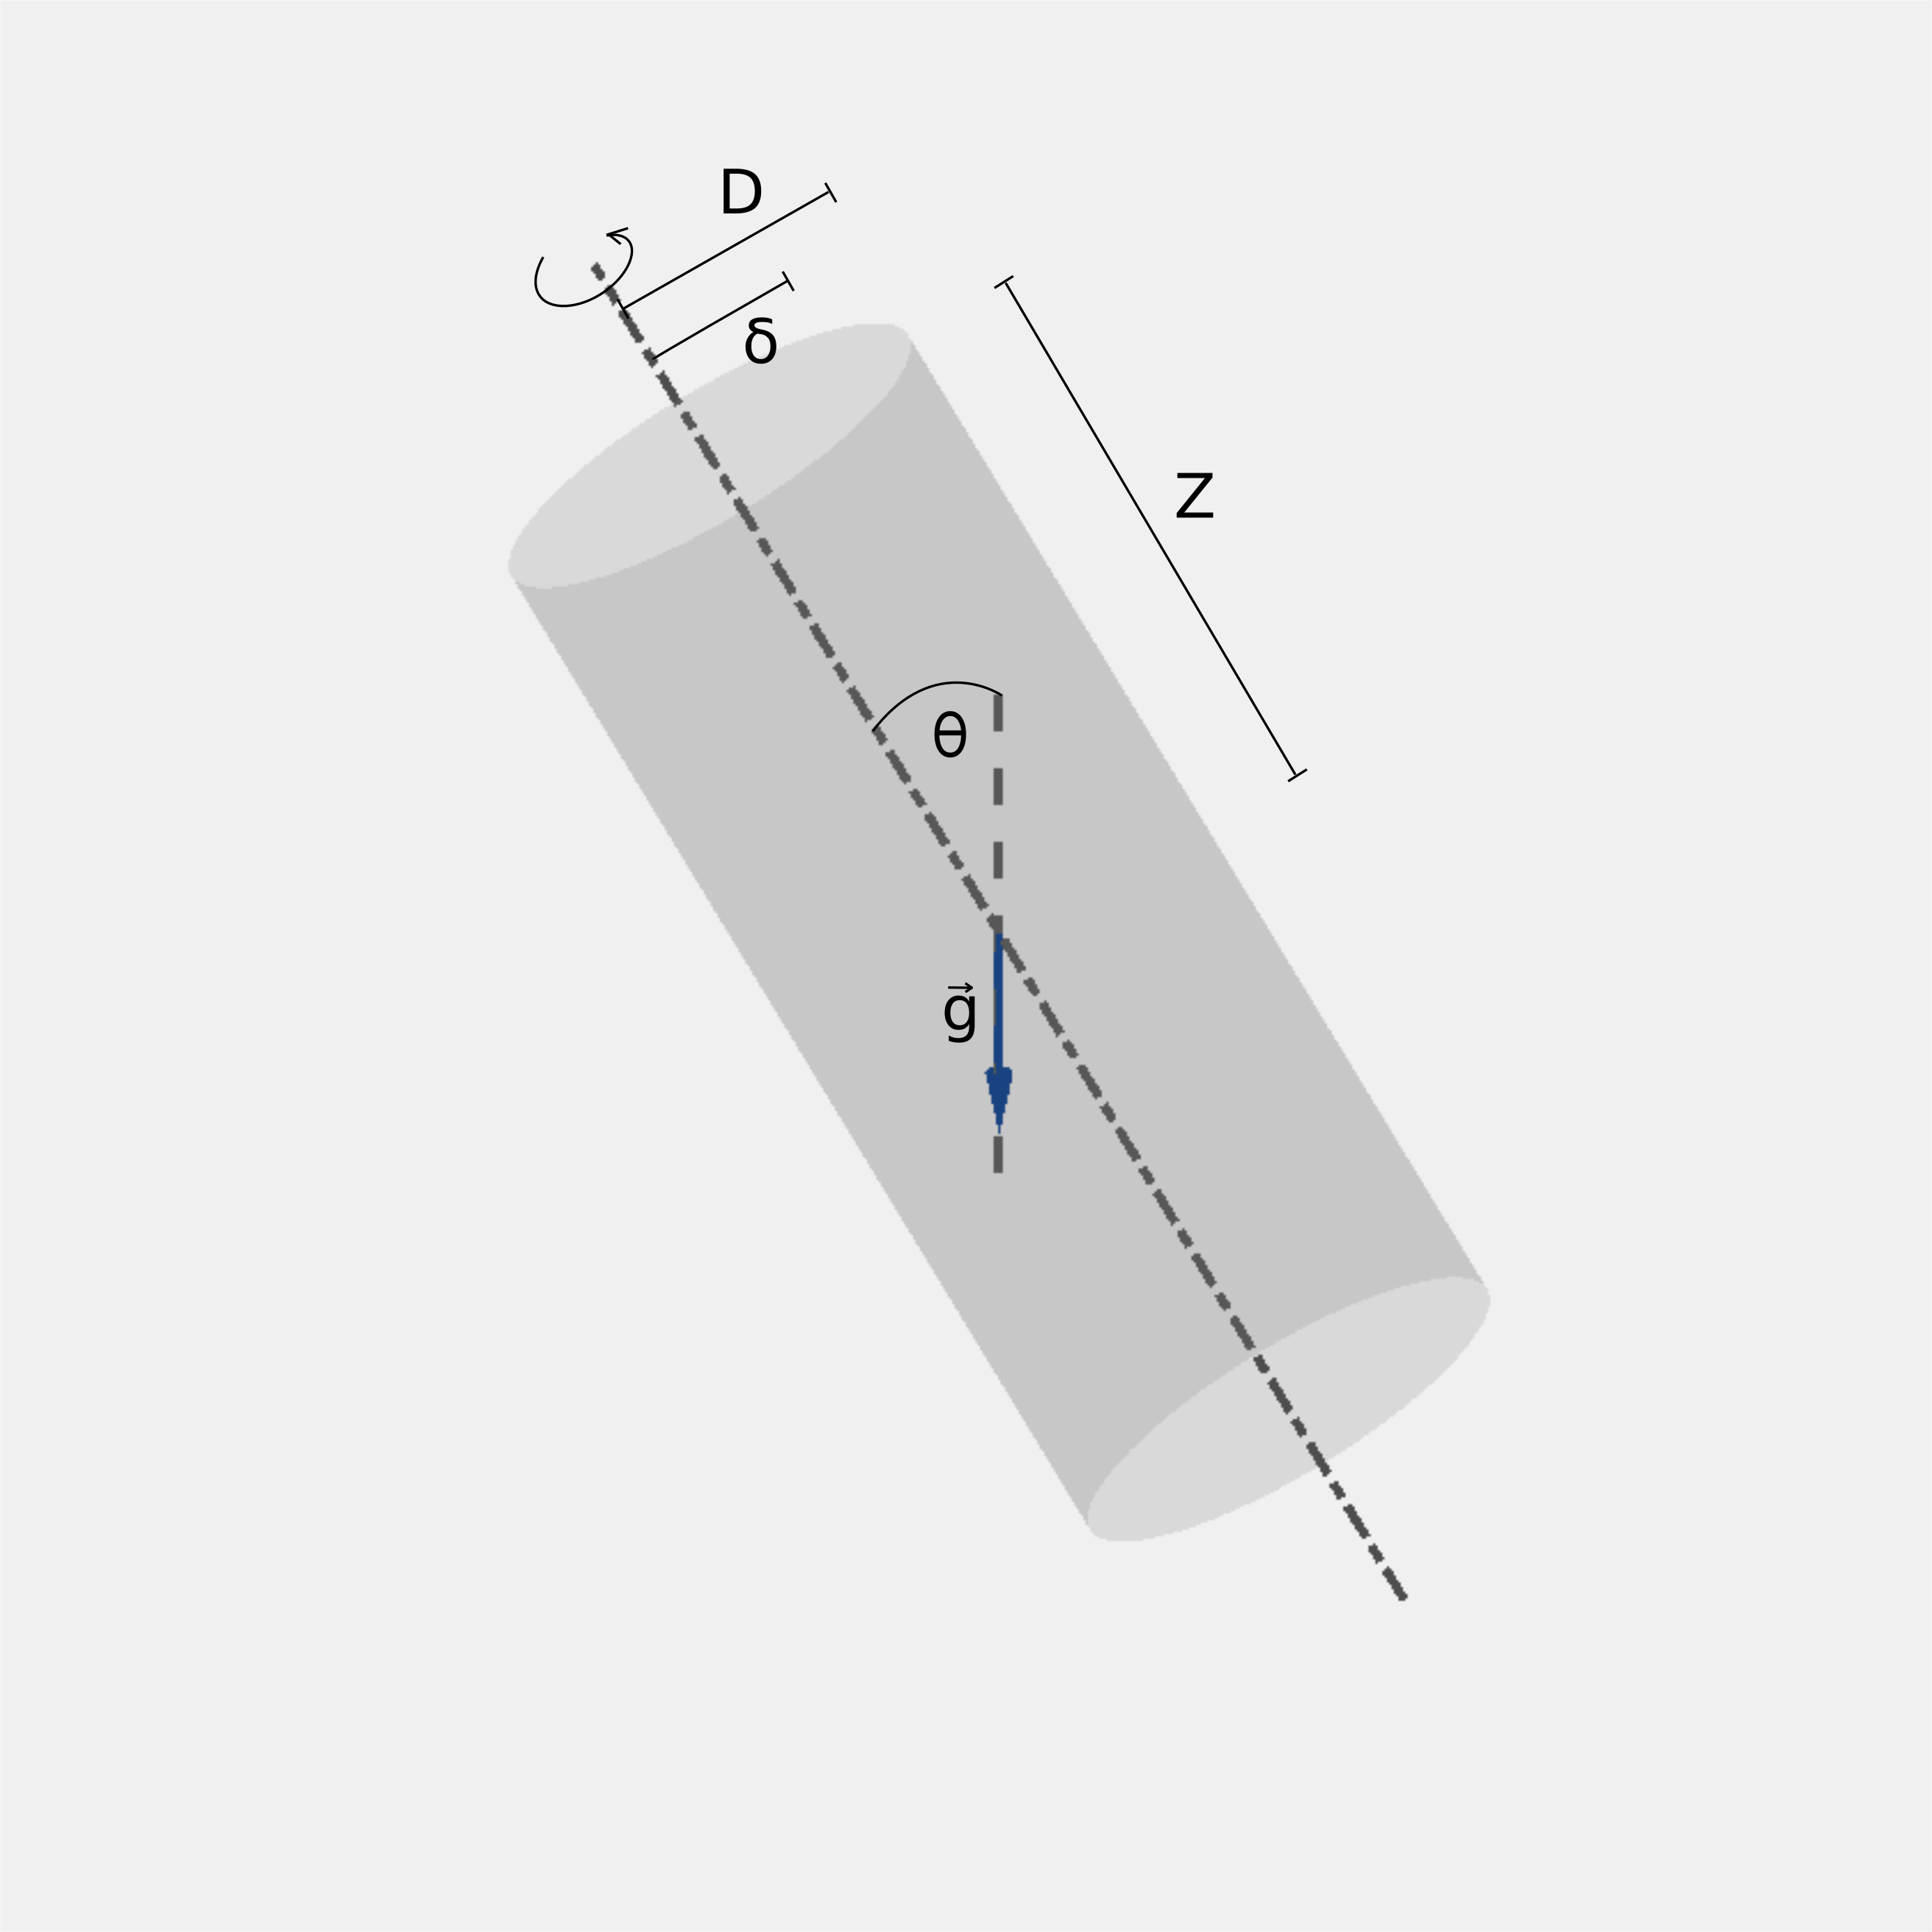
\includegraphics[width=20pc]{gfx/vortex_domain.png}
\caption{A scheme of numerical simulation's vortex model domain. $D$ is cylider radius, $Z$ is its half-length, $\delta$ is vortex core size, $\theta$ is gravity alignment angle, $\vec{g}$ is gravity direction.}
\label{fig:ch2_05}
\end{figure*}
New particles are constantly placed in the simulation domain in the following way. Cylinder shell of constant width $\Delta r_{box}=200 \mu m$ (chosen as a compromise between largest particle size and grid accuracy) is discretized by imposing a rectangular grid on it, where one grid box has real dimensions $(\Delta r_{box},\Delta \varphi_{box},\Delta z_{box})$ and volume $V_{box}$.

\begin{align}
\Delta r_{box}=\Delta z_{box}=200 \mu m, \\
\Delta \varphi_{box}= \Delta r_{box}/D,\\
V_{box}=\Delta r_{box}^3,\\
\vec{v}_{box}=\vec{u}_r(r=D)=-\gamma D/2 \ \hat{e_r},\\
\/i N_i=n*V_{box},\\
\Delta t_{box}=\Delta r_{box}/|\vec{v}_{box}|=2 \Delta r_{box}(\gamma D)^{-1}.
\end{align}

Initial particle velocity $\vec{v}_{box}$ is set to equal fluid radial stretching velocity at cylinder surface. Initial positions of the new particles are generated on the grid with number density $n$ and randomized with homogeneous spatial distribution, so the probability of having a particle in an arbitrary $i$-th box is the same for all the boxes and equals $N_i$. New particles are placed in the shell at time intervals of equal duration $\Delta t_{box}$. The initiation of new particles is designed in such a manner to somehow connect the vortex domain with an external environment where the concentration of particles is assumed to be $n$ as well.

Tu moze jeszcze bedzie fragment o tym jak sie zmienia liczba czastek w czasie w roznych symulacjach.\\

 Droplet number concentration within the domain is almost constant and the pattern does not change. After a few seconds, each simulation becomes steady.

\section{Cloud voids observation}
\label{ch2s4}

Observations of the already mentioned cloud structures called cloud voids were performed with the use of lasersheet photography technique. They were accompanied by simultaneous measurement of turbulence and cloud droplet properties. The details of the lasersheet technique and turbulence methods are outlined below in subsequent subsections.\\
Observations were performed on 27 and 29 August 2011 at
Umweltforschungsstation Schneefernerhaus (UFS) on the
slopes of Zugspitze in the German Alps. Each time, the cloud event lasted for several hours. Figure \ref{fig:ch2_06} presents the measurement setup on UFS roof. For a detailed description of the observatory and characterization of the usual cloud and turbulence conditions on site, see \citet{Risius2015} and \citet{Siebert2015}. Authors of these papers showed that turbulence and cloud microphysical properties at the measurement site are quite reasonable representations of measurements made in “free” clouds away from the surface.\\
\begin{figure*}
\centering
\noindent \includegraphics[width=30pc]{gfx/Zugspitze_view.png}
\caption{Upper part of the figure presents an image of UFS observatory on the slope of Zugspitze. Lower part shows the arrangement of instuments at the UFS roof.}
\label{fig:ch2_06}
\end{figure*}

\subsection{Atmospheric turbulence measurements}
High-resolution measurements of small-scale turbulence during cloud void events were performed by 3D ultrasonic anemometers operated at 10~Hz, providing digital outputs for three components of wind velocity $\vec{u}=(u,v,w)$, where $u$ and $v$ are horizontal components and $w$ is vertical velocity. Having 3D velocity, the mean wind velocity and its fluctuations are estimated in appropriately selected time intervals (also by running average). The time series is treated as spatial series on the basis of Taylor’s frozen-flow hypothesis. Velocity fluctuations' 2nd order structure functions are calculated. The Kolmogorov "2/3 law" formulated for the structure functions (Eq. \ref{def:struct_fun_inertial}) determines mean energy dissipation rate $\langle\epsilon\rangle$ and further the Kolmogorov spatial scale $\langle\eta\rangle$.\\
Droplet size distribution was measured by a phase Doppler interferometer (PDI) probe mounted approximately 6~m down from the cloud voids observation point. The principle of the device is based on heterodyne detection of Doppler-shifted light from individual droplets, that results in a robust measurement of the droplet diameter and a single component of the droplet velocity vector \citep{Chuang2008}.\\
Relative humidity and temperature measurements were conducted on-site as well. Relative humidity during cloud immersion was around 100\%. More on cloud microphysical properties measurements can be found in \citet{Siebert2015}.\\

\subsection{Lasersheet photography}

In laserheet photography particles are illuminated by a sheet of laser light. A camera placed at a certain angle to this plane collects images of the light scattered by the particles. In general, particle image recorded by the camera depends on the incoming light, the mutual position of the light sheet and the camera sensor, sensor properties and the nature of scattering process itself. Firstly, the light incident on the particle is characterized by its spectrum and spatial structure of the incident beam, what depends on the particle position with respect to width, length and divergence of laser sheet. Secondly, the camera sensor pixel responds with a signal registration only if it receives an amount of energy exceeding a certain threshold. The amount of light received by the camera depends on aperture and exposure time. Light scattered by a particle passes through the optics and undergoes some transformations, specific to a camera. What is more, the particle image on the sensor is characterized by the internal intensity distribution (diffraction pattern). All this influences single pixel signal intensity. Image size depends on particle size, optics’ magnification, position with respect to the focus and other factors\citep{Olsen2000}. Thirdly, the scattered light intensity at an arbitrary angle depends nonlinearly on particle size when comes to light scattering on cloud-like particles. A larger particle can give a lower scattered intensity than a smaller one, or there may be several orders of magnitude difference in intensity between particles differing by one order of magnitude in size. The scattering theory applied for cloud droplets and visible light is called Mie theory and is summarised next.\\
The Mie scattering theory is a rigorous mathematical theory describing the problem of elastic scattering of light by a dielectric sphere of arbitrary size and homogeneous refractive index in the case in which a sphere size is similar to or larger than the wavelength of the incident light. It shows a complex angular and particle size dependency of the scattered light intensity (van de Hulst, 1957). Figure \ref{fig:ch_07} presents this dependency for chosen parameter ranges. Thus, brightness of images of laserlight scattered by polydisperse set of droplets is not expected to be monotonic with the particle size.

\begin{figure*}
\centering
\noindent 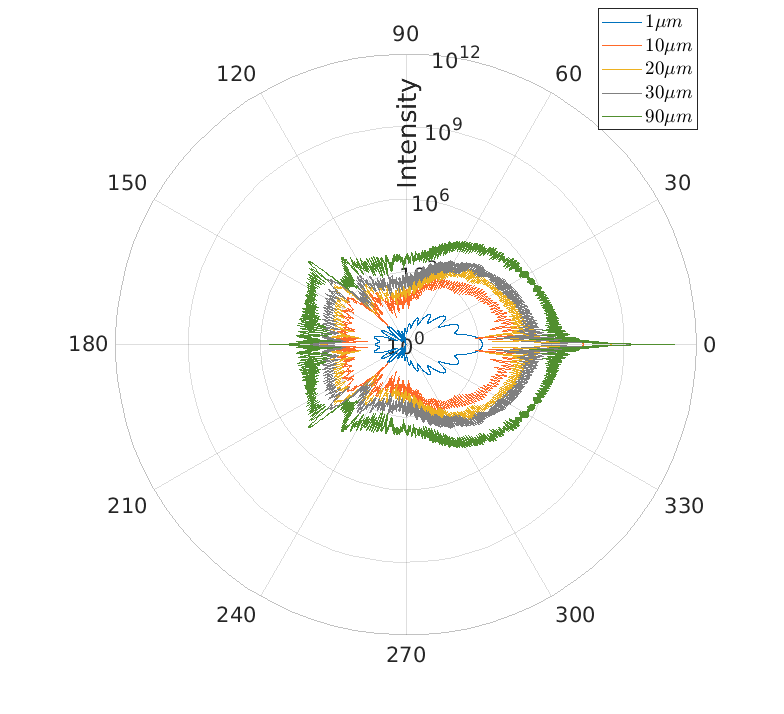
\includegraphics[width=20pc]{gfx/I_vs_angle_multiple.png}
\caption{Relative intensity of scattered light (on radial axis, in logarithmic scale) on scattering angle and sphere radius according to Mie scattering theory.}
\label{fig:ch2_07}
\end{figure*}

In cloud void observations in 2011 clouds were illuminated by a laser sheet created with a frequency-doubled high-power Nd:YAG laser (532~nm, 45~W). The sheet was set either vertical or oblique with respect to gravity. The angle between the laser sheet plane and camera recording plane in the oblique case was chosen to increase the scattering intensity on droplets and falls within the range of 30–40~$\deg$. The laser sheet in the observation region was around 50~cm wide and 1~cm thick. Images covering the approximately 2~m long section of the sheet at a distance approximately 10~m from the source were taken with a Nikon D3s 12 MP DSLR camera. Figure \ref{fig:ch2_08} shows an example of an unprocessed image.

\begin{figure*}
\centering
\noindent 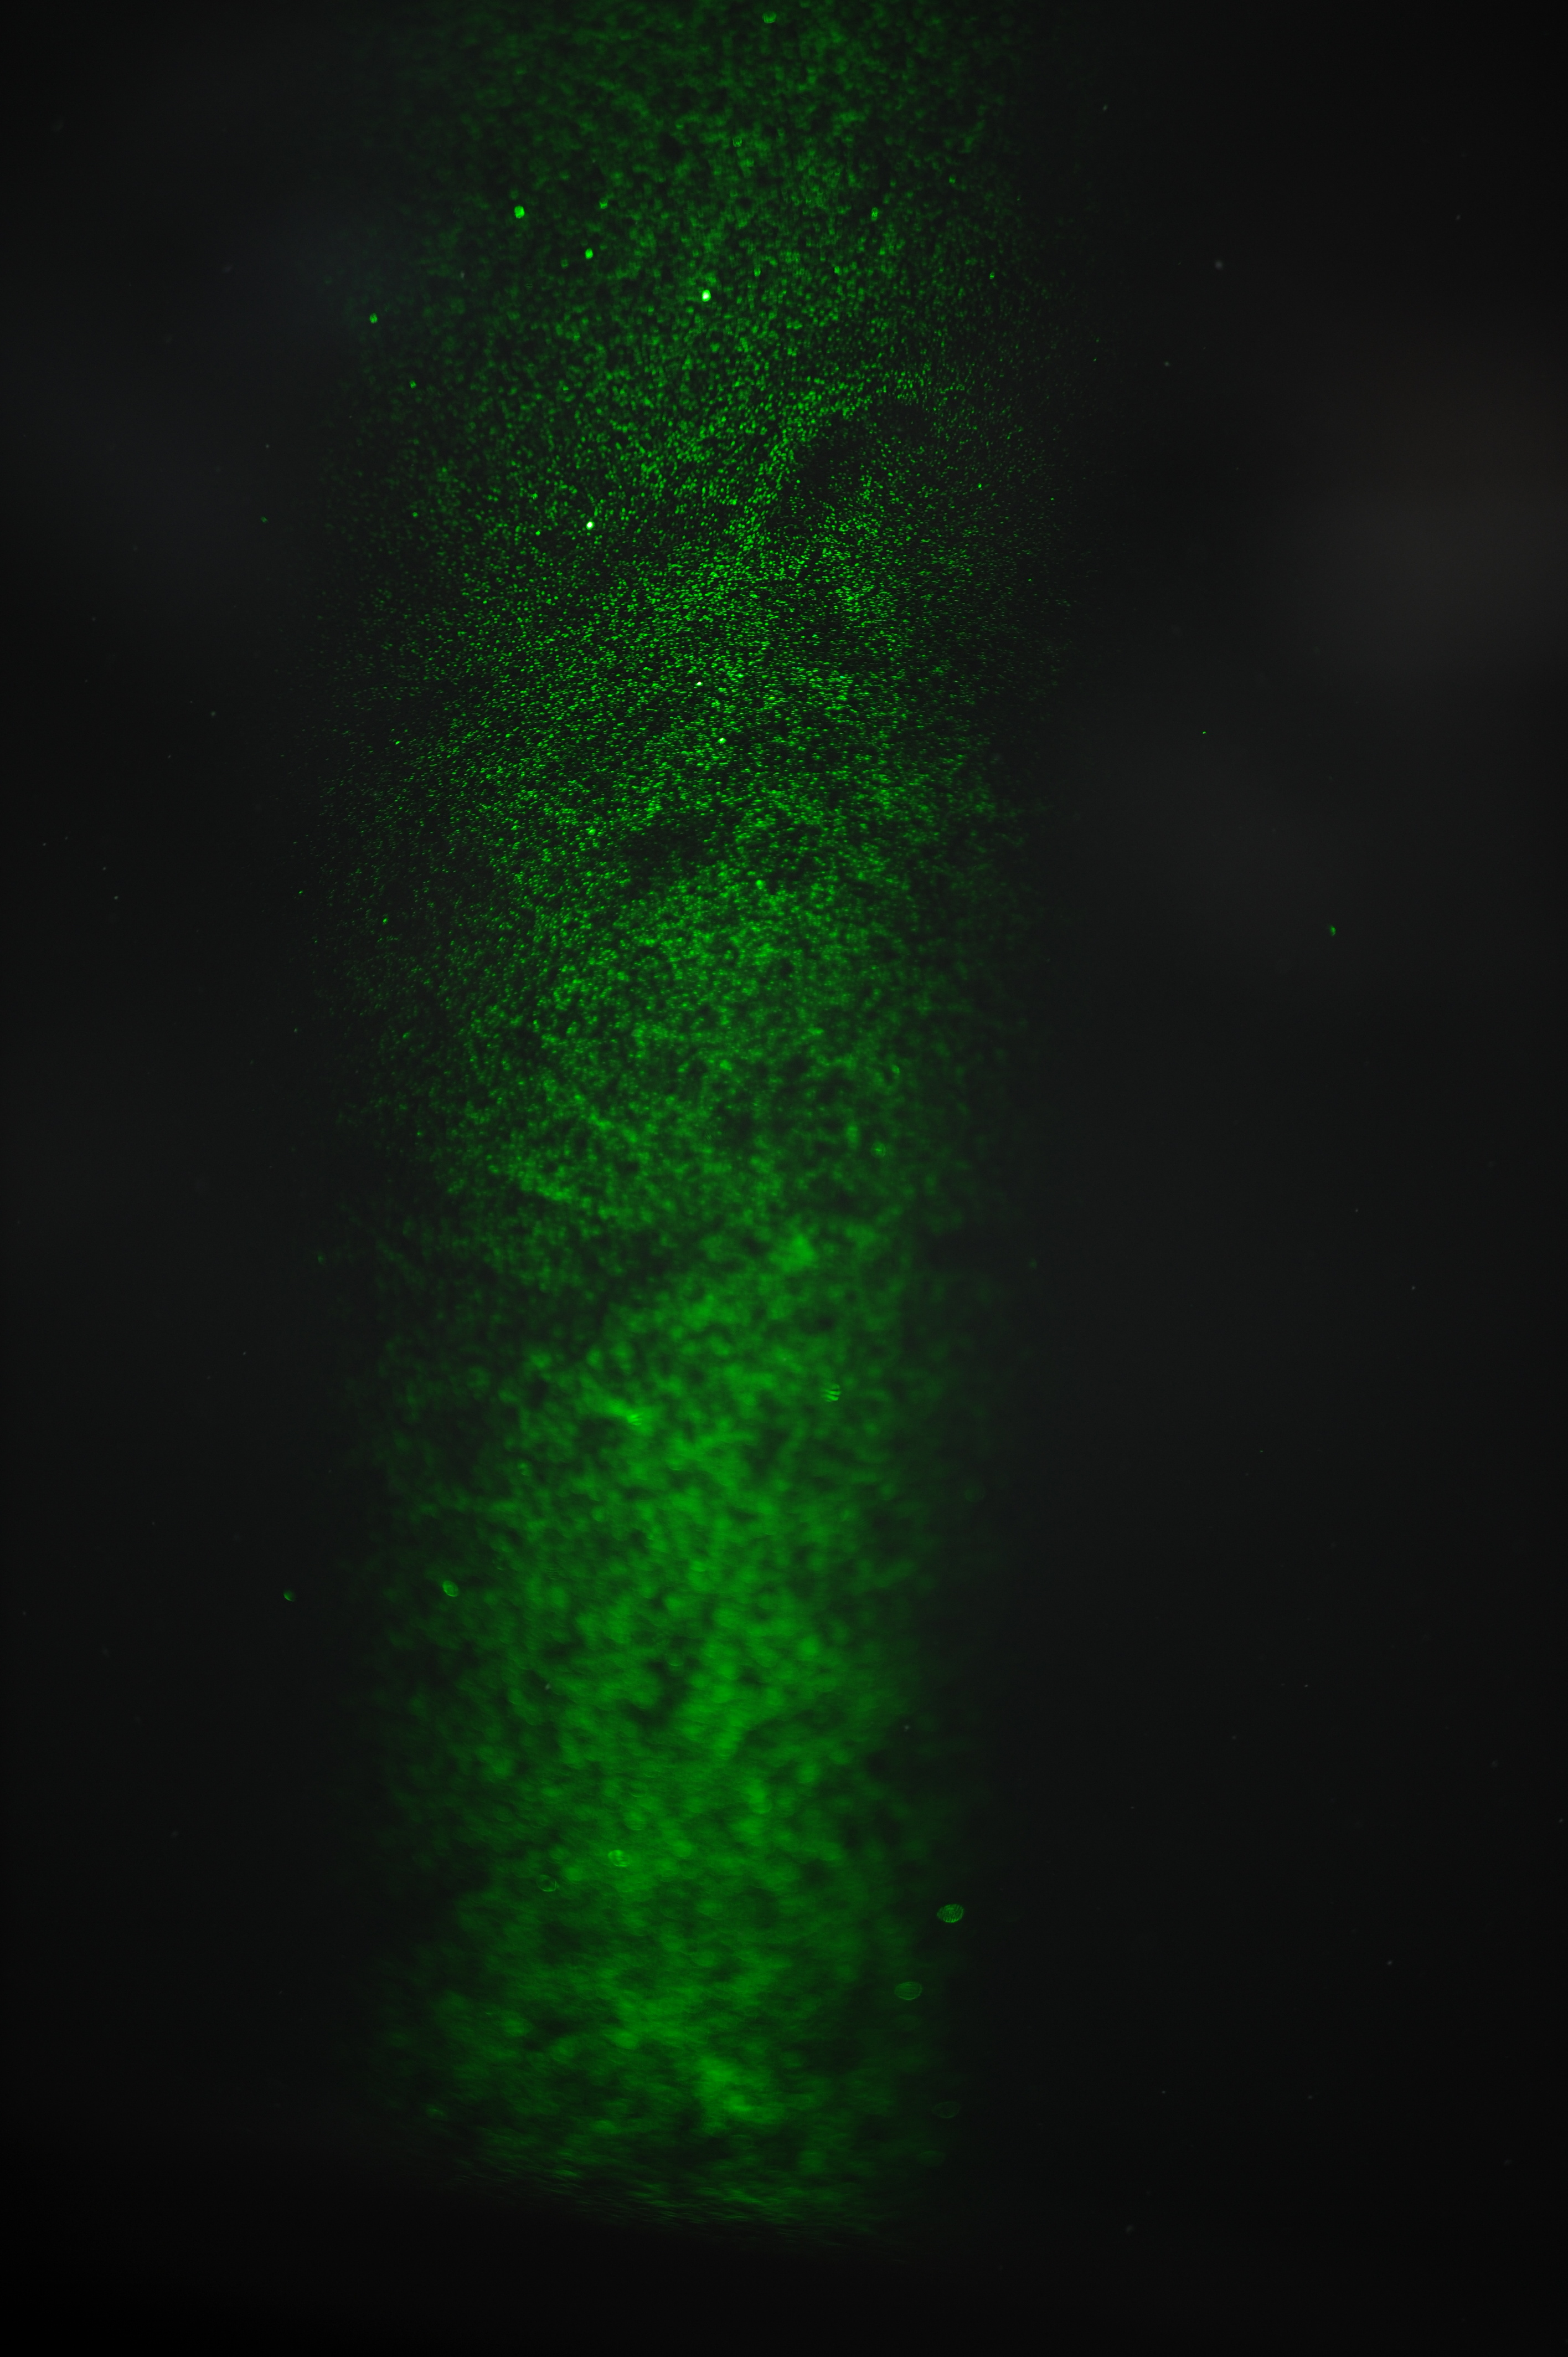
\includegraphics[width=20pc]{gfx/imaging_example_1617.jpg}
\caption{Image of mountain-top cloud particles, illuminated by a laser sheet light (Nd:YAG laser, 532~nm, 45~W), taken at 8:24~AM on 27th of August 2011 by Markus Neumann. Exposure time: 1/3200~s,focal length: 200~mm, f/2.8.}
\label{fig:ch2_08}
\end{figure*}

Aquired images were used for size estimation of cloud voids, i.e. small (a few centimeters’ scale) clear-air regions in cloud droplet field of round or elliptic shapes. Each one’s size was manually determined. In the case of a round void, the diameter was taken as the size; in the case of flattened or ellipsoidal void, the maximal chord was taken. The imprecise setting of the measurement system does not allow to evaluate the influence of the lasersheet geometry on droplet imaging in and around cloud voids.  \\
In order to compare measurements with the results of the numerical simulations, a simplified procedure of droplet size scaling and color scaling, including the effects of laser imaging technique, is proposed. For this purpose, the following assumptions are made:
\begin{itemize}
\item one particle image is recorded by one pixel,
\item the signal received by a pixel changes linearly with incident light intensity only,
\item each particle is in focus and its image size depends linearly on the particle size,
\item the experiment in clouds was set up to allow best visualization of maximal number of particles possible.
\end{itemize}
Calculation of the Mie scattering intensity is performed with the help of an algorithm that was described in \citet{Bohren2007}. The scattering angle corresponds to 40~$\deg$. In the size range of cloud particles, the light intensity has a general growing tendency, but it is still strongly nonlinear. There are 3 orders of magnitude difference between particles of 1 and 30~$\mu m$ radius. Relative intensity is calculated on this basis. Next, the brightness scaling is made. It assumes that experiment was set up to enable visualization of 95~\% of particle size spectrum. The particle size at which the cumulant of the particle size distribution reaches 95~\% was calculated. Particles larger than this size have brightness equal to 1 in the simulation visualisations. Brightness for the other particles scales linearly with relative scattered light intensity. To mimic camera sensitivity, there is a threshold below which particles get brightness equal to 0. In the plot with white background, the relation is opposite, so the brightest particles are black, and the least bright are white. This color scaling was used in Section \ref{} of Chapter \ref{} for numerical simulation plots and calculations.\\
Dwa zdania o próbie z ramka swiatła (opcjonalnie).

\section{Cloud-like conditions}
\label{ch2s5}

In order to draw meaningful conclusions from numerical experiments, it is necessary to determine the parameter space for the simulations. In this case, cloud particle and turbulence data is needed, what is further called "cloud-like" conditions. However simultaneuos measurements of cloud droplet microphysics and tubulence properties, as stated before, are scarce. Here, some data collected in various clouds during different experiments are presented. Table \ref{tab:ch2_01} contains basic variables, such as mean TKE dissipation rate $\langle\epsilon\rangle$, $\eta$ calulated with the use of mean dissipation rate, Tylor microscale Reynolds number $Re_{\lambda}$ (calculated according to Eq.\ref{def:Tylor_scale}), droplet radius range $R$, mean droplet radius $\langle R \rangle$ and mean concentration. It is important to remember that mean values estimations may significantly differ between papers. Fig.\ref{fig:ch2_09} presents in addition the Stokes number $St$ and settling parameter $S_v$ space corresponding to some data in Table \ref{tab:ch2_01}.

\begin{table}[h!]
\centering
\begin{tabular}{|l|l|c|c|c|c|c|c|c|} 
\hline
lala & unit & \multicolumn{3}{|c|}{UFS, Zugspitze \citep{Siebert2015}} & \multicolumn{2}{|c|}{POST \citep{Jen-LaPlante2016}} & \multicolumn{2}{|c|}{CARRIBA \citep{Siebert2013}}\\ [0.5ex]
\hline \hline
 clouds & - & no clouds & small Cu$^{c}$, thin Sc$^{c}$ & Sc$^{c}$ & Sc$^{m}$ TISL & Sc$^{m}$ CTMSL & \multicolumn{2}{|c|}{shallow Cu$^{m}$}  \\ 
$\langle\epsilon\rangle$ & $m^2 s^{-3}$ & $8.5 \cdot 10^{-2}$ & $10^{-1}$ & $10^{-1}$  & $0.07-0.32\cdot 10^{-3}$ &$0.38-1.46\cdot 10^{-3}$ & $2\cdot 10^{-3}$ & $3\cdot 10^{-3}$\\
$\eta$ & mm & 0.4 & - & - & 2.39-3.32 &1.24-1.78 & - & - \\
$Re_{\lambda}$& - & 6200 & - & - &- & - & - & -\\
$R$ & $\mu m $ & - & 2.5-10 & 3-17 & - & - & 4-47 & 4-45\\ 
$\langle R \rangle$ & $\mu m$ & - & 4.45 & 6.45 & - & -& 19 & 13.5\\
$\langle n \rangle$ & $cm^{-3}$ & - & 532 &  275 & - &-& 42 & 80 \\ [1ex] 
 \hline
\multicolumn{8}{l}{$^{c}$ - continental, $^{m}$ - maritime clouds}
 \end{tabular}
 \label{tab:ch2_01}
\end{table}


\begin{table}
\centering
\refstepcounter{table}
\label{tab:ch2_01}
\resizebox{\linewidth}{!}{%
\begin{tabular}{|>{\hspace{0pt}}p{0.131\linewidth}|>{\hspace{0pt}}p{0.081\linewidth}|>{\centering\hspace{0pt}}p{0.106\linewidth}|>{\centering\hspace{0pt}}p{0.145\linewidth}|>{\centering\hspace{0pt}}p{0.064\linewidth}|>{\centering\hspace{0pt}}p{0.127\linewidth}|>{\centering\hspace{0pt}}p{0.129\linewidth}|>{\centering\hspace{0pt}}p{0.091\linewidth}|>{\centering\arraybackslash\hspace{0pt}}p{0.091\linewidth}|} 
\toprule
lala                      & unit          & \multicolumn{3}{>{\centering\hspace{0pt}}p{0.315\linewidth}|}{UFS, Zugspitze Siebert2015} & \multicolumn{2}{>{\centering\hspace{0pt}}p{0.256\linewidth}|}{POST Jen-LaPlante2016} & \multicolumn{2}{>{\centering\arraybackslash\hspace{0pt}}p{0.182\linewidth}|}{CARRIBA Siebert2013}  \\ 
\hhline{|=-=======|}
{[}0.5ex] clouds          & -             & no clouds            & small Cu$^{c}$, thin Sc$^{c}$  & Sc$^{c}$                          & Sc$^{m}$ TISL             & Sc$^{m}$ CTMSL                                           & \multicolumn{2}{>{\centering\arraybackslash\hspace{0pt}}p{0.182\linewidth}|}{shallow Cu$^{m}$ }    \\
$\langle\epsilon\rangle$  & $m^2 s^{-3}$  & $8.5 \cdot 10^{-2}$  & $10^{-1}$                      & $10^{-1}$                         & $0.07-0.32\cdot 10^{-3}$  & $0.38-1.46\cdot 10^{-3}$                                 & $2\cdot 10^{-3}$  & $3\cdot 10^{-3}$                                                               \\
$\eta$                    & mm            & 0.4                  & -                              & -                                 & 2.39-3.32                 & 1.24-1.78                                                & -                 & -                                                                              \\
$Re_{\lambda}$            & -             & 6200                 & -                              & -                                 & -                         & -                                                        & -                 & -                                                                              \\
$R$                       & $\mu m $      & -                    & 2.5-10                         & 3-17                              & -                         & -                                                        & 4-47              & 4-45                                                                           \\
$\langle R \rangle$       & $\mu m$       & -                    & 4.45                           & 6.45                              & -                         & -                                                        & 19                & 13.5                                                                           \\
$\langle n \rangle$       & $cm^{-3}$     & -                    & 532                            & 275                               & -                         & -                                                        & 42                & 80                                                                             \\
\bottomrule
\end{tabular}
}
\end{table}

\begin{figure*}
\centering
\noindent 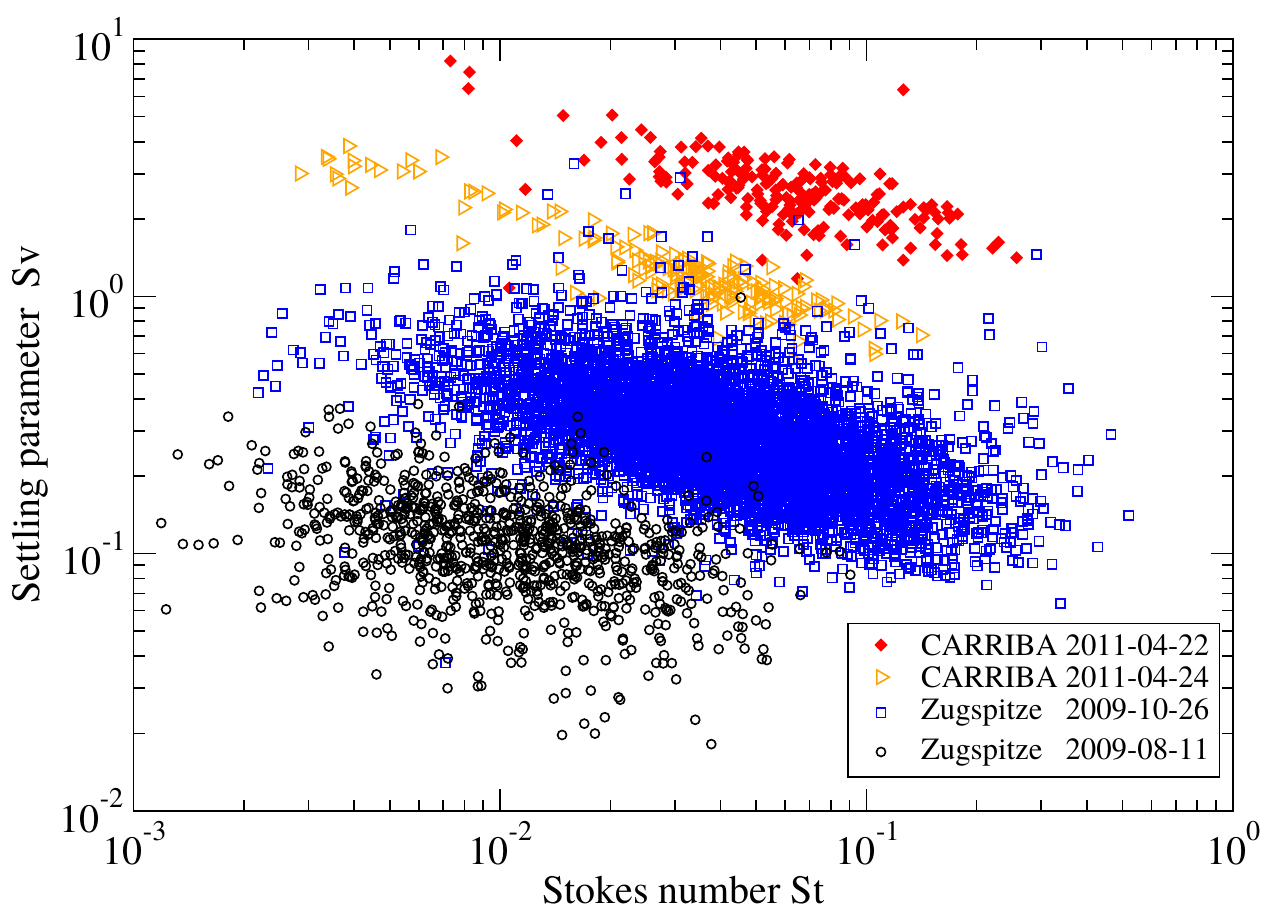
\includegraphics[width=30pc]{gfx/Sv_vs_St_experimental_Siebert2015.png}
\caption{Stokes number $St$ and settling parameter $S_v$ space. Each point is based on a 1~s average of cloud data. The CARRIBA data represent typical conditions for clean (red) and slightly more polluted (yellow) cases and provide a reference for typical trade wind cumuli (see \citep{Siebert2013} for more details). Reprinted from \citep{Siebert2015}.}
\label{fig:ch2_09}
\end{figure*}

 
%  $\nu$ & $m^2 s^{-1}$ & - &  &  \\
%  $\mu$ & $kg \ m^{-1} s^{-1}$ & - &  &  \\
%  $\rho_p$ & $kg \ m^{-3}$ & - &  &  \\
%  $\rho_f$ & $kg \ m^{-3}$ & - &  &  \\
%  $g$ & $m s^{-2}$ & - &  &  \\
\end{document}